\documentclass[a4]{article}
\usepackage[utf8]{inputenc}
\usepackage[french]{babel}
\usepackage{listings}
\usepackage{color}
\usepackage{graphicx}
\usepackage[T1]{fontenc}
\usepackage{pdfpages}
\usepackage{geometry}
\geometry{hmargin=2.5cm,vmargin=2.5cm}

\definecolor{mygreen}{rgb}{0,0.6,0}
\definecolor{mygray}{rgb}{0.5,0.5,0.5}
\definecolor{mymauve}{rgb}{0.58,0,0.82}

\lstset{
  backgroundcolor=\color{white},   % choose the background color; you must add \usepackage{color} or \usepackage{xcolor}
  basicstyle=\footnotesize,        % the size of the fonts that are used for the code
  breakatwhitespace=false,         % sets if automatic breaks should only happen at whitespace
  breaklines=true,                 % sets automatic line breaking
  captionpos=b,                    % sets the caption-position to bottom
  commentstyle=\color{mygreen},    % comment style
  deletekeywords={...},            % if you want to delete keywords from the given language
  escapeinside={\%*}{*)},          % if you want to add LaTeX within your code
  extendedchars=true,              % lets you use non-ASCII characters; for 8-bits encodings only, does not work with UTF-8
  frame=L,	                       % adds a frame around the code
  keepspaces=true,                 % keeps spaces in text, useful for keeping indentation of code (possibly needs columns=flexible)
  keywordstyle=\color{blue},       % keyword style
  language=C,                 	   % the language of the code
  otherkeywords={*,...},           % if you want to add more keywords to the set
  numbers=none,                    % where to put the line-numbers; possible values are (none, left, right)
  numbersep=5pt,                   % how far the line-numbers are from the code
  numberstyle=\tiny\color{mygray}, % the style that is used for the line-numbers
  rulecolor=\color{black},         % if not set, the frame-color may be changed on line-breaks within not-black text (e.g. comments (green here))
  showspaces=false,                % show spaces everywhere adding particular underscores; it overrides 'showstringspaces'
  showstringspaces=false,          % underline spaces within strings only
  showtabs=false,                  % show tabs within strings adding particular underscores
  stepnumber=2,                    % the step between two line-numbers. If it's 1, each line will be numbered
  stringstyle=\color{mymauve},     % string literal style
  tabsize=2,	                   % sets default tabsize to 2 spaces
  title=\lstname                   % show the filename of files included with \lstinputlisting; also try caption= instead of title
}
%gestion des caractères latins
\lstset{literate=
  {á}{{\'a}}1 {é}{{\'e}}1 {í}{{\'i}}1 {ó}{{\'o}}1 {ú}{{\'u}}1
  {Á}{{\'A}}1 {É}{{\'E}}1 {Í}{{\'I}}1 {Ó}{{\'O}}1 {Ú}{{\'U}}1
  {à}{{\`a}}1 {è}{{\`e}}1 {ì}{{\`i}}1 {ò}{{\`o}}1 {ù}{{\`u}}1
  {À}{{\`A}}1 {È}{{\'E}}1 {Ì}{{\`I}}1 {Ò}{{\`O}}1 {Ù}{{\`U}}1
  {ä}{{\"a}}1 {ë}{{\"e}}1 {ï}{{\"i}}1 {ö}{{\"o}}1 {ü}{{\"u}}1
  {Ä}{{\"A}}1 {Ë}{{\"E}}1 {Ï}{{\"I}}1 {Ö}{{\"O}}1 {Ü}{{\"U}}1
  {â}{{\^a}}1 {ê}{{\^e}}1 {î}{{\^i}}1 {ô}{{\^o}}1 {û}{{\^u}}1
  {Â}{{\^A}}1 {Ê}{{\^E}}1 {Î}{{\^I}}1 {Ô}{{\^O}}1 {Û}{{\^U}}1
  {œ}{{\oe}}1 {Œ}{{\OE}}1 {æ}{{\ae}}1 {Æ}{{\AE}}1 {ß}{{\ss}}1
  {ű}{{\H{u}}}1 {Ű}{{\H{U}}}1 {ő}{{\H{o}}}1 {Ő}{{\H{O}}}1
  {ç}{{\c c}}1 {Ç}{{\c C}}1 {ø}{{\o}}1 {å}{{\r a}}1 {Å}{{\r A}}1
  {€}{{\EUR}}1 {£}{{\pounds}}1
}
%definition d'un syle pour les documents text
\lstdefinestyle{txt}{
	frame=none,
	numbers=none,
	stringstyle=\color{black},
}

\begin{document}
	\title{\Huge{\textbf{Cahier Des Specifications}}}
	\author{Alabi Steve - Benyamna Younes - Capdenat Nicolas- \\
		Chouipe Thibaut - El Harti Zakaria - Lienhardt Florian \\ \\ \\
		Chef de projet : Benyamna Younes \\ \\ \\ 
		Sous la direction de Mme Kloul \\ \\ \\ \\
		Outil automatique de décryptage \\ \\ \\}
		

	\begin{titlepage}
		\maketitle
		\vspace{20em}
		\begin{center}
\includegraphics{logo_uvsq.jpg}\end{center}
	\end{titlepage}
	\section{Introduction}
Dans le cadre de notre troisième année de licence nous devons réaliser une application d'aide au
décryptage par la méthode de Substitution ainsi que celle de Vigenère.
Nous vous avons donc proposé l'application Dcrypt qui permet de décrypter 
mais également crypter un text ou même de faire une analyse fréquentielle sur un text.
Pour cela, nous avons rédigé un cahier des charges afin de clarifier les objectifs et les 
exigences de ce projet. Dans la suite du cahier des charges, nous vous proposons donc
le cahier des spécifications.\\

Pour développer notre projet et après étude des besoins les arguments en faveur du langage C sont les suivants:\\

-Tout d'abord, le C permet d'utiliser des expressions et des opérateurs qui sont très proches du langage machine, 
il est donc possible de développer des programmes efficients et rapides.\\

-La portabilité est aussi un argument de choix: En effet, en respectant le standard ANSI-C, il est possible d'utiliser
le même programme sur tout autre système (autre hardware, autre système d'exploitation), simplement en le recompilant.\\

-De plus, pour assurer la maintenance du produit apres sa realisation et ce meme par des developpeurs qui ne sont
pas ceux d'origine, il faut un langage des plus utilisés et maitrisés\\

-Enfin, selon l'IEEE(*), le langage C est depuis 2016 le meilleur langage de 
programmation( de par sa forte croissance et sa demande par les employeurs). C'est aussi le langage n=1 pour le développement
d’applications d’entreprise, de bureau et d'applications scientifiques.\\

Nous avons également choisi une bibliothèque graphique du langage C: GTK+. Cette dernière nous permet de gérer efficacement
la navigation entre les differentes fenêtres
ainsi que nos accès memoires pour la sauvegarde et le chargement de nos fichiers. 
IEEE(*):  Institut des ingénieurs électriciens et électroniciens.
C'est la plus grande organisation professionnelle technique du monde de l'évolution de la technologie
	\section{Organigramme}
			\underline{Interface graphique :}     \hspace{5cm}  \underline{Cryptage Substitution :}\\
			- bouton cryptage            \hspace{5.5cm}       -créer une clé aleatoirement\\
			- bouton decryptage         \hspace{5cm}        -crypter le message\\
			- bouton substitution\\
			- bouton Vigenère           \hspace{5.2cm}       \underline{Cryptage Vigenère :}\\
			- affichage de text(complet et partiel)  \hspace{2.2cm} -crypter le message\\
			- affichage pour la clé de substitution\\
			- bouton Francais(decryptage)   \hspace{3.5cm}     \underline{Decryptage Substitution :}\\
			- bouton Anglais(decryptage)    \hspace{3.5cm}     -decrypter le message\\
			- affichage pour l'analyse fréquentielle\\
			- charger un fichier text       \hspace{4.2cm}  \underline{Analyse fréquentielle :}\\
			- sauvegarder un fichier text     \hspace{3.8cm}  -analyse frequentielle sur text donné\\
			- créer un nouveau fichier text(resultats)\\
			- Demander clef de Vigenère\\
			
			
			\underline{Decryptage Vigenère :}\\
			-decrypter le message\\
			

			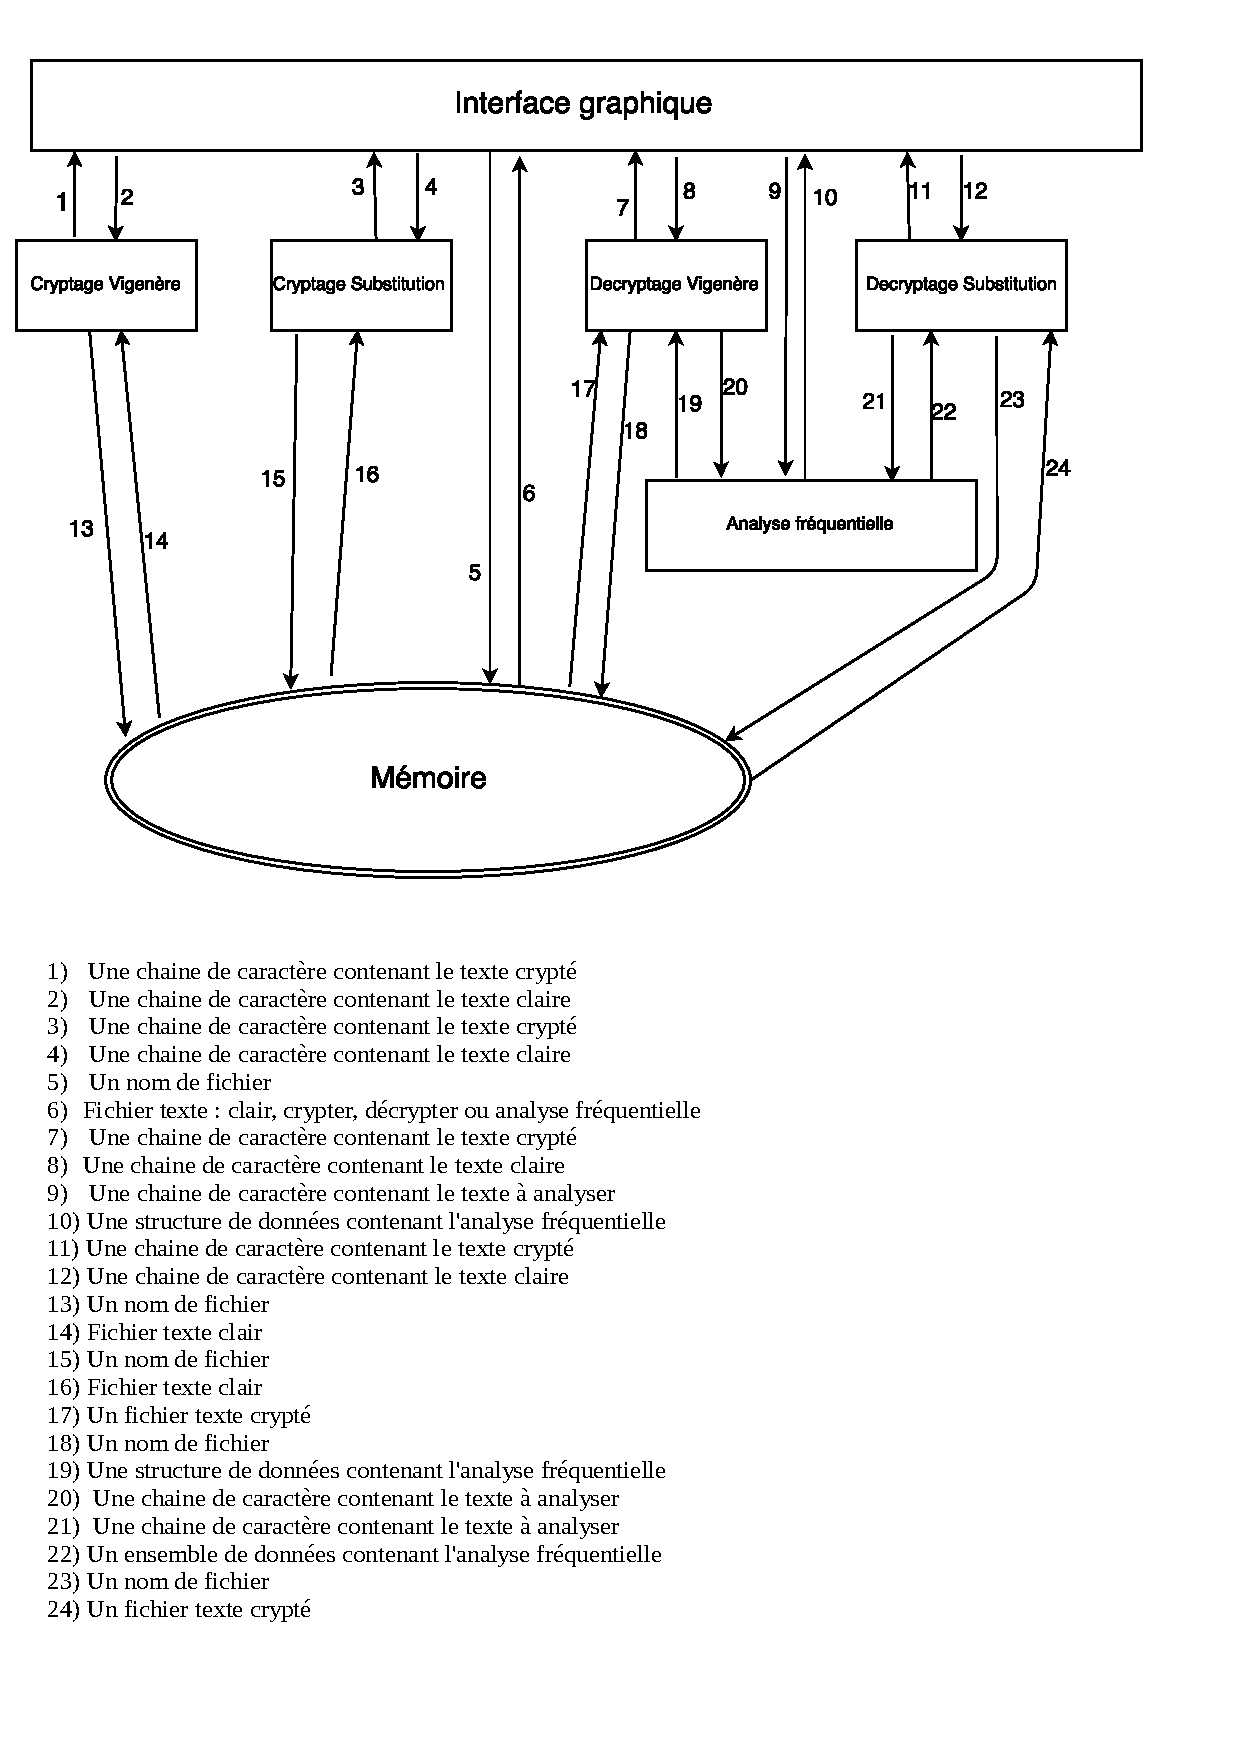
\includepdf[scale=0.7]{organ.pdf}
			
			
	\section{Signatures et Explications des methodes}
		\subsection{Diagramme des fonctions des differents modules}
								Le diagramme résume les fonctions/procédures présentes dans chaque module ainsi que les liens d'inclusion.\\

		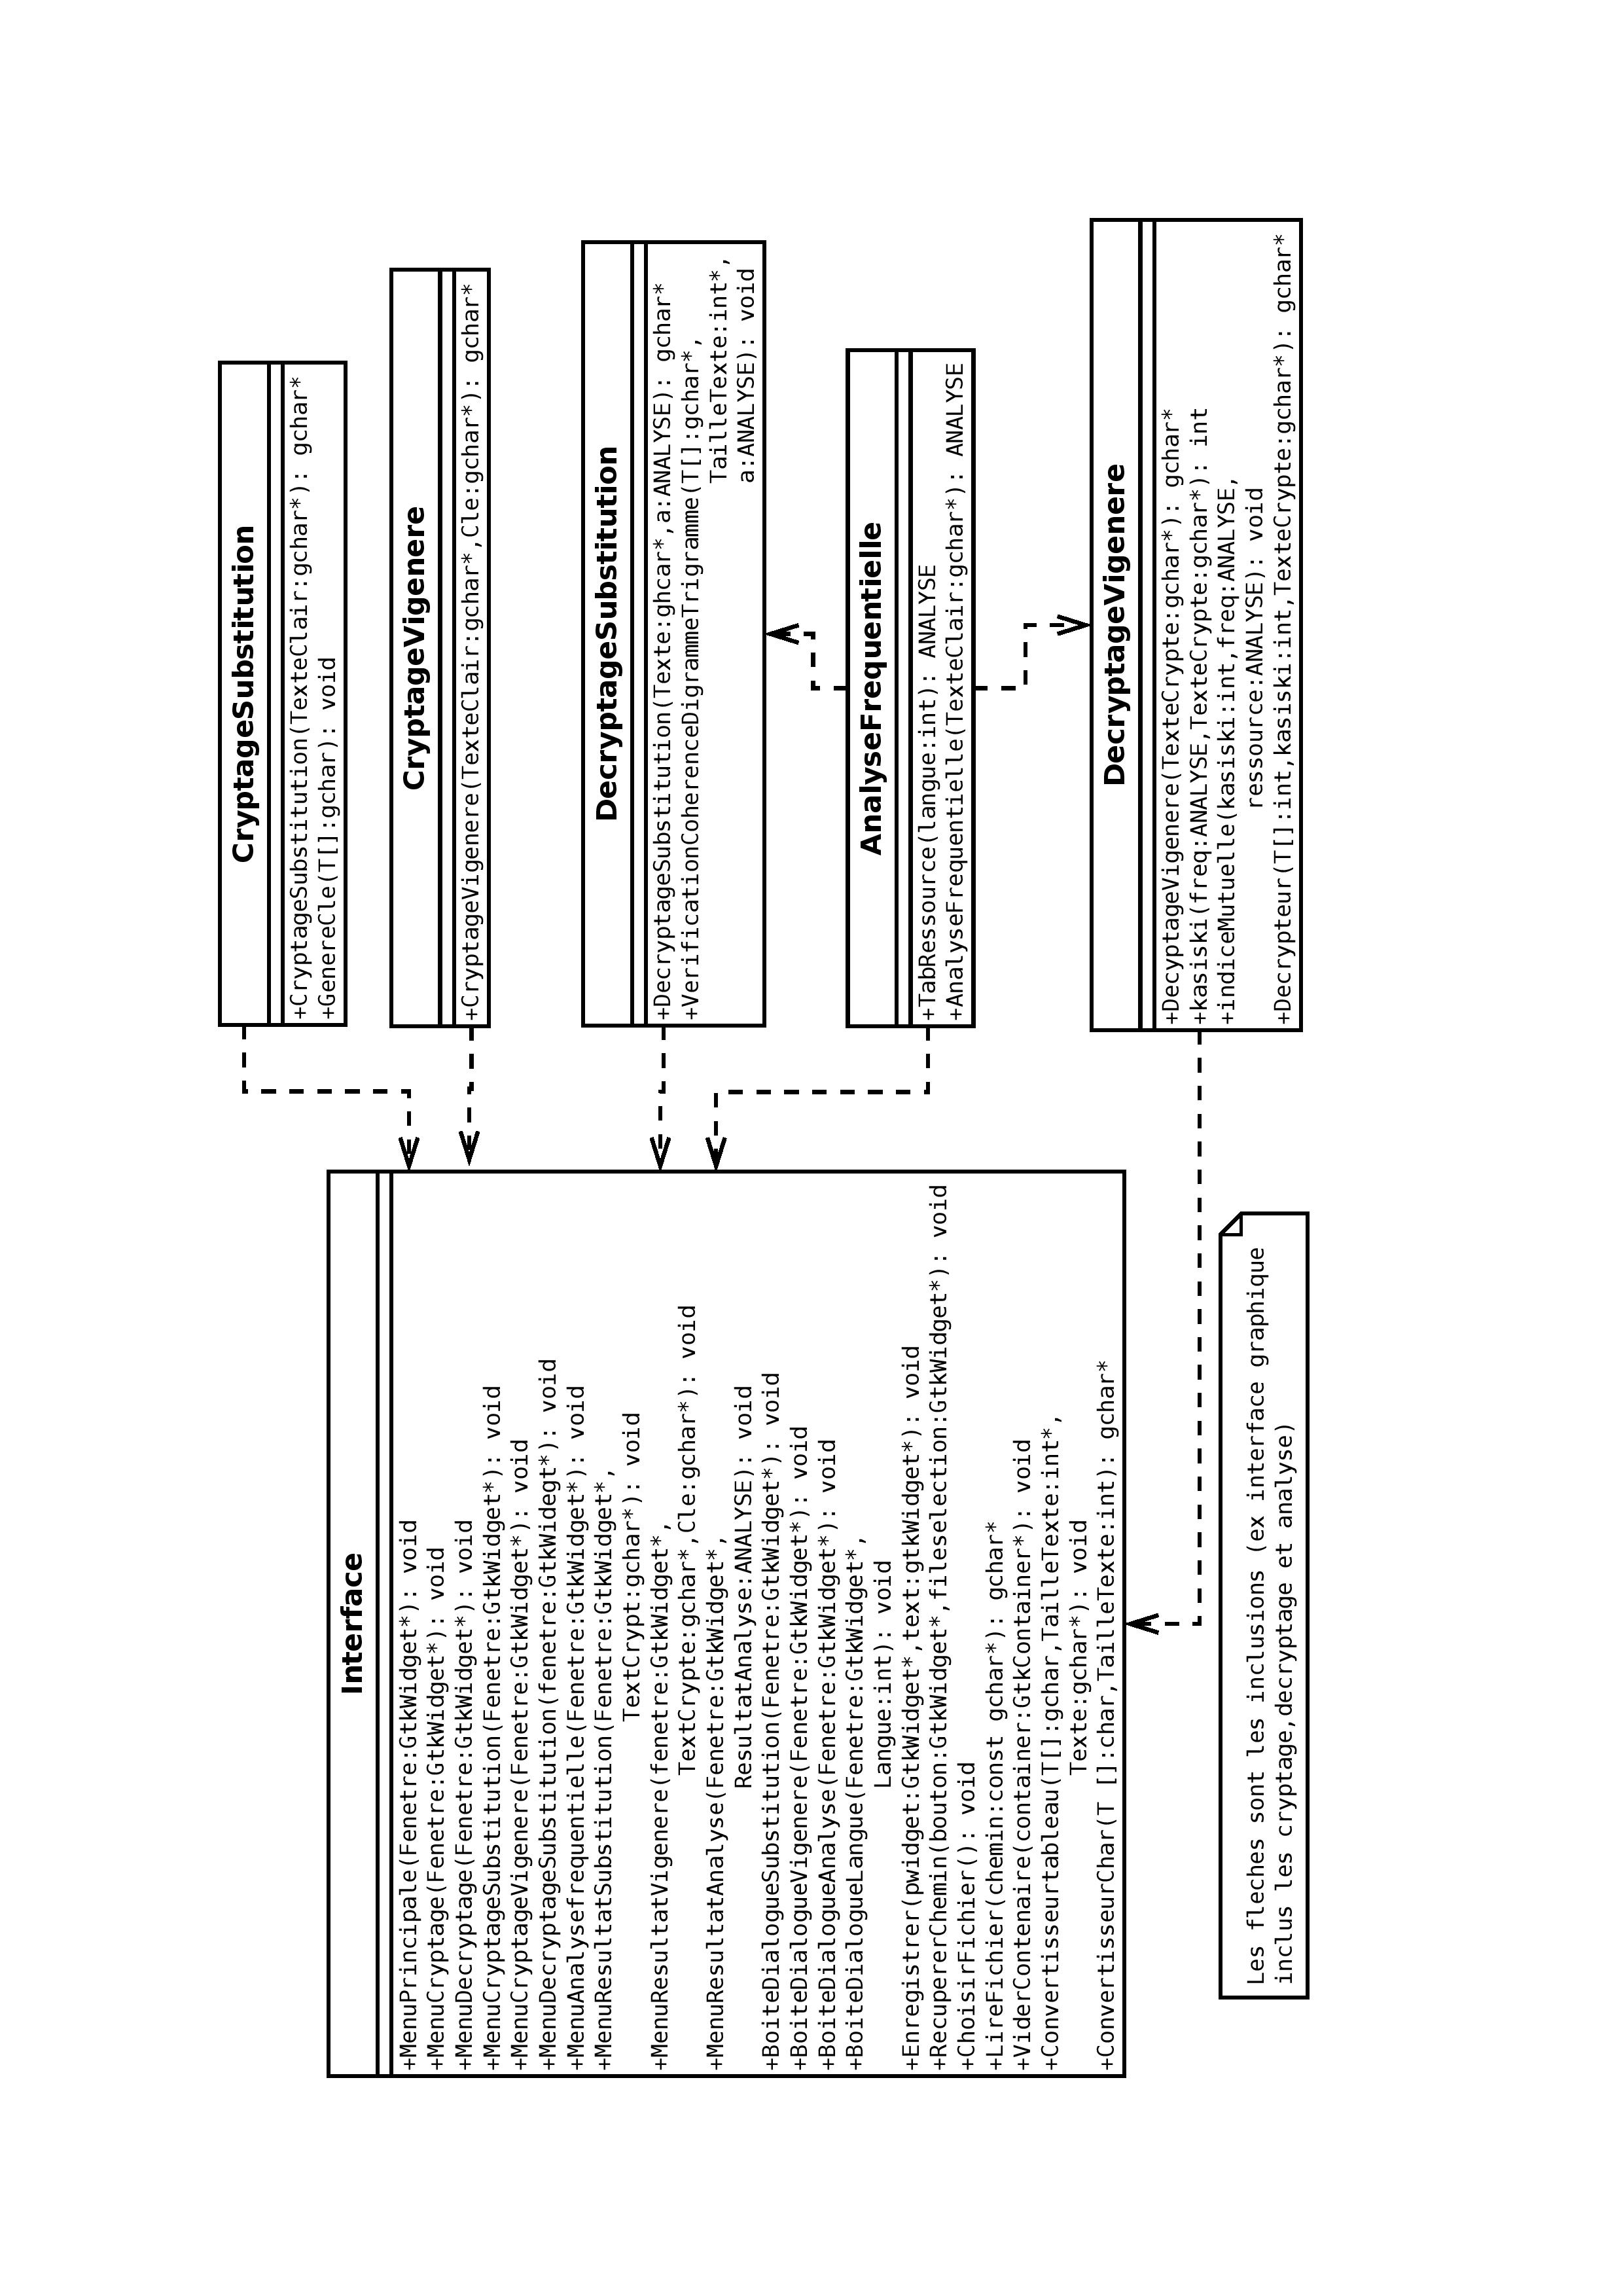
\includegraphics[scale=0.8]{diaa.jpg}
		\subsection{Structures et nouveaux types}
		Le gchar* est une chaîne de caractères, on utilise pas char* car dans la bibliothèque
		GTK+ l'affichage d'un text se fait avec gchar*.\\
		
		les widgets (GTKWidget) sont les boutons, les zones de text, les menus, enfin.. à peu 
		près tout ce qui constitue une interface.\\
		
		L'argument "gchar* TextClair" que l'on va retrouver par la suite dans plusieurs fonctions
		designe le texte clair(le texte lisible).\\
		
		Les variables globales utilisées dans notre programme sont Fenetre et Langue. Fenetre nous permet de
		conserver la fenêtre principale de notre application:\\
		GtkWidget *Fenetre; \\
		Langue permet, quant a elle, de garder la langue utilisée.
		int Langue;\\
		
		
		
	typedef struct phoneme\{\\
		int frequence;\\
		gchar* nom;\\
	\}PHONEME;\\
	Cette structure représente les digrammes ou trigrammes et leurs fréquences.\\
	"nom" représente le nom du phoneme et la frequence est le nombre d'occurences\\
	de ce dernier.\\
	
	typedef struct analyse\{ \\
		int nb; \\
		float occ[25];\\
		PHONEME di[20];\\
		PHONEME tr[20];\\
		gchar* pgor;\\
	\}ANALYSE;\\
	Cette structure correspond aux caractéristiques d'un text. Elle sera remplie lors de
	l'appel de la fonction "AnalyseFrequentielle". Ainsi, on connaitra
	le nombre de caractères dans celui-ci, les digrammes/trigrammes, la plus grande occurence
	rencontrée et la frequence d'apparition de chaque lettre.\\
	le nb représente le nombre de lettres dans le texte etudié, occ est un tableau qui contient \\
	le nombre d'occurences de chaque lettre (occ[0] pour A etc..) ,di et tr contiennent les digrammes \\
	et les trigrammes dans le texte ainsi que leurs nombres d'occurences.\\
	pgor est la chaine de caracteres qui contiend la Plus Grande Occurance Rencontrée dans notre texte .\\
	
	
	typedef struct ressourceslangue\{ \\
		float occ[25];\\
		PHONEME di[20];\\
		PHONEME tr[20];\\
	\}RESSOURCESLANGUE;\\
	Cette structure correspond aux caractéristiques d'une langue. On connaitra
	les digrammes/trigrammes et la fréquence d'apparition de chaque lettre dans la langue choisie.\\
	occ est un tableau qui contient le nombre d'occurences de chaque lettre (occ[0] pour A etc..) \\
	,di et tr contiennent les digrammes et les trigrammes dans le texte ainsi que leurs nombre d'occurences.
		\subsection{Signatures}
		
	
	\subsubsection{Analyse Frequentielle}
	RESSOURCESLANGUES TabRessource();\\
		La fonction recupère un entier correspondant à la langue(francais ou anglais, en variable globale)
		et va ainsi remplir la structure "RESSOURCESLANGUES" et ses attributs suivants:
		la fréquence d'apparition de chaque lettre dans la langue choisie ainsi que les digrammes
		et les trigrammes.\\
		Elle renvoie la structure RESSOURCESLANGUES remplie.
		
	ANALYSE AnalyseFrequentielle(gchar* TextCrypté)\\
		La fonction prend en entrée le text crypté à analyser et va ainsi remplir la structure "ANALYSE" et 
		ses attributs suivants:
		le nombre de lettres, la fréquence d'apparition de chaque lettre, les digrammes, les trigrammes
		et la plus grande occurence rencontrée. Ils seront logiquement remplis en fonction du texte.\\
		Elle renvoie la structure ANALYSE remplie.
		
	\subsubsection{Cryptage Substitution}
	gchar* CryptageSubstitution(gchar* TextClair);\\
		Cette fonction permet de crypter un text avec la méthode de Substitution\\
		Pour cela, elle prend en entrée une chaine de caractères qui correspond au text clair.\\
		On utilise ensuite la fonction "ConvertisseurTableau".
		Le text à crypter se trouve alors dans un tableau que nous allons parcourir. Et pour chaque caractere 
		nous allons lire dans un autre tableau [2][26] où la premiere ligne du tableau([0][]) correspond à l'alphabet
		de base et la deuxième ligne ([1][]) celui de substitution(le nouveau).Que l'on aura generé à l'aide de la fonction "GenereCle". Ainsi, nous regardons la lettre dans 
		le premier tableau ( celui du texte à crypter), on bascule dans le deuxieme tableau et trouve ce caractere dans la première ligne, puis on regarde sa lettre de substitution (2e ligne) et enfin on remplace dans le premier tableau 
		la lettre de base par ce caractère de substitution. En sortie, le text crypté sera sous forme de chaine de caractères grace à la fonction "ConvertisseurChar".
		
	void GenereCle(gchar T[]);\\
		Cette procédure permet de génerer une clé(alphabet) aléatoirement. On la modifie à l'aide de pointeurs.
	
	\subsubsection{Decryptage Substitution}
void DecryptageSubstitution( gchar* texteCrypté)
	Cette fonction prend en argument une chaine de caractère contenant le texte crypté.
	Elle va commencer par appeler la fonction convertisseurtableau qui va stocker les  caractères 
	du texte crypté dans un tableau. 
	DecryptageSubstitution va ensuite appeler les fonctions AnalyseFrequentielle et TabRessource. 
	Aprés avoir appelé ces 	fonctions elle va, dans une boucle comparer les résultats de l'analyse frequentielle stockés 		dans une structure ANALYSE créée par AnalyseFrequentielle aux données stockées dans une structure RESSOURCESLANGUE créée 	 grace à la fonction TabRessource et contenant une analyse fréquentielle sur l'alphabet correspondant à la langue 		choisie(anglais ou francais).
	Elle va alors remplacer dans le tableau une lettre du message crypté par la lettre qu'elle semble crypter grace à une 		conjecture basée sur les fréquences des lettres les plus utilisées et complétée par l'analyse des digrammes et 			trigrammes, elle va egalement crée une clef de substitution sous la forme d'un tableau de caractère de la taille de 		l'alphabet (la premiére case correspondra au caractère décryptant la lettre A, la seconde au caractère décryptant la 		lettre B ect...).
	Cette fonction appellera ensuite la fonction VerificationCoherenceDigrammeTrigramme.
	La boucle prendra fin lorsque la clef de substitution sera complète, c'est à dire quand tous les caractères
	de l'alphabet seront décryptés.
	Cette fonction ne renverra rien puisque son but va être de permettre l'affichage du décryptage et de la clef de 		décryptage pendant et à la fin de l'opération.
	Cette affichage sera appelé dans lafonction VerificationCoherenceDigrammeTrigramme.


	void VerificationCoherenceDigrammeTrigramme( gchar T[], int TailleTexte, gchar clef[], int TailleAlphabet, 
	RESSOURCESLANGUE Ressource)
	Prend en argument un tableau T de la taille du texte crypté et contenant le texte crypté en cours de
	décryptage, une structure RESSOURCESLANGUE crée grace à la fonction contenant une analyse fréquentielle sur 
	l'alphabet correspondant à la langue choisit(anglais ou francais) ainsi qu'un tableau clef de la
	taille de l'alphabet et correspondant à la clef de substitution.
	Cette fonction vas parcourir le texte en cours de décryptage pour vériffier que les letres trouvé ne forme pas de 
	digramme ou trigramme inabituelle. Si c'est le cas elle proposera à l'utilisateur de corriger le décryptage du texte ou 
	le corrigera d'elle même. Pour se faire elle appelera la fonction ConvertisseurChar afin de stocké le résultat du texte 
	partiellement décrypté dans une chaine de caractère permettant son affichage grace à la fonction 		
	MenuResultatDecryptagePartiel la fonction appeller pourra également récupérer la clef de substitution final ainsi que le
	texte final afin de les enregistrer. Ainsi l'utilisation de cette fonction suivra deux ca de figures: soit la fonction 
	ne détécte aucune anomalie est les tableaux en entrée ne sont pas modifiés, soit elle détécte des anomalies et les 	
	tableau sont alors modifiés avec l'aide de l'utilisateur.
	
	
	\subsubsection{Decryptage Vigenère}
	gchar* DecryptageVigenere(gchar* textCrypte, gchar* safecle);\\
		Cette fonction prend en argument un texte crypté par le chiffrement de Vigenère ainsi 
		que safecle (chaine de caractères) qui va permettre de sauvegarder la clé.
		Appels des fonctions AnalyseFrequentielle et TabRessource qui vont initialisées les valeurs 
		contenue dans la structure ANALYSE ainsi que convertisseurtableau qui va stocker le texte crypté 
		dans un tableau.
		Ensuite appelle la fonction Kasiski qui va conjecturée la taille de la clé.
		Puis, on déclare un tableau cle[taillekasiski] de taille correspondant à la fonction kasiski. 
		On appelle la fonction indiceMutuelle qui remplira les valeurs des caractères de la clé dans le tableau cle[]
		ainsi que safecle qui contient les caractères mêmes.\\
		On appelle la fonction Decrypteur, cette dernière nous servant à retourner le texte en clair.\\
	
	int Kasiski(ANALYSE freq, gchar* texteCrypte);\\
		Cette fonction prend une structure ANALYSE en argument afin de connaitre le 
		PGOR (Plus Grande Occurence Rencontrée) et/ou les trigrammes,ainsi que le texteCrypte à décrypter.
		Elle cherche les différentes distances de PGOR et effectue le PGCD de ces distances.
		Elle renvoie ce résultat sous forme d'un entier (qui représente la taille du mot clé cherché).\\
	
	void indiceMutuelle(int cle[],int kasiski, ANALYSE freq, ANALYSE ressource, gchar* safecle);\\
		Cette fonction prend en argument le tableau clé qui contiendra les valeurs de notre mot clé,
		freq qui contient les fréquences de chacune des lettres du textes et ressource la
		probabilité d'apparition d'une lettre dans la langue choisie.
		Cette fonction calcule les indices de coïncidences mutuelles et les enregistrent dans un tableau tab[25][kasiski].\\
		Elle parcourt et compare les 26 valeurs de chaque ligne afin de reperer celles qui sont proches de 0,065
		(une par ligne).\\
		Elle modifie le tableau cle[] passé en argument qui contiendra l'indice de chacunes des valeurs choisies dans un 
		tableau à une dimension et affecte a safecle la clé afin de pouvoir l'afficher dans le menu. \\
	
	gchar* Decrypteur( int cle[], int kasiski, gchar* texteCrypte);\\
		Cette fonction prend en argument le tableau cle ainsi que le texte a décrypter.
		Elle va soustraire la valeur du mot clef (tableau renvoyé par indiceMutuelle) au texte crypté.\\
		Elle va répeter la suite de nombre composant le mot clef (contenue dans le tableau passé en argument) jusqu'a
		la fin du texte afin de toujours pouvoir soustraire une valeur du mot clé a une valeur du texte crypté.\\
		Elle renvoie le texte en clair, c'est a dire décrypté.\\
		
		\subsubsection{Cryptage Vigenère}
	gchar* CryptageVigenere(gchar* texteClair, gchar* Cle);\\
		Cette fonction permet de crypter un texte avec la methode de Vigenère\\
		Elle prend en argument le texte clair et la clé qui sont tout les deux des chaines de caractères.\\
		On construit un tableau [3][taille texte]. En première ligne([0][]) on trouvera le texte a crypter(ou plutot la valeur en entier de chaque caractere du texte a crypter), 
		en 2e ligne([1][]) la clé (qu'on repetera de facon a couvrir toute la 1e ligne et donc le message a chiffrer). La aussi chaque caractere de la clé sera directement inscrit en entier et enfin en 3e ligne([2][]) le resultat de l'addition des caracteres(entiers) des deux premieres lignes le tout modulo 26.
		On lira toute cette derniere ligne (l'entier de chaque case) et on ira remplir un second tableau avec directement le caractere correspondant a cet entier.
		La fonction "ConvertisseurChar" permettra de renvoyer le texte crypté sous forme de gchar*.
		
		\subsubsection{Interface Graphique}
		Dans ce module nous allons utiliser plusieurs menus pour afficher notre application et naviguer 
		entre les menus pour cela nous allons créer plusieurs procédures qui vont afficher les menus  
		
		\textit{Les Menus}\\
		
		Toutes le procedure suivante ne renvoie rien et elle prennent en argument un conteneur(c'est l'endroit où sera affiché le contenu present dans ce menu)
		
	void MenuPrincipal(GtkWidget *Fenetre);\\
		Cette procédure permet d'afficher le menu principal.\\
		Elle prend en argument la fenetre qui sera le contenaire(des boutons et labels).\\
	
	void MenuCryptage(GtkWidget *Fenetre);\\
		Cette procédure permet d'afficher le menu de cryptage.\\
		Elle prend en argument la fenetre qui sera le contenaire(des boutons et labels).\\

	
	void MenuDecryptage(GtkWidget *Fenetre);\\
		Cette procédure permet d'afficher le menu de decryptage.\\
		Elle prend en argument la fenetre qui sera le contenaire(des boutons et labels).\\

	
	void MenuCryptageSubstitution(GtkWidget *Fenetre);\\
		Cette procédure permet d'afficher le menu de cryptage par la méthode de substitution.\\
		Elle prend en argument la fenetre qui sera le contenaire(des boutons et labels).\\

	
	void MenuCryptageVigenere(GtkWidget *Fenetre);\\
		Cette procédure permet d'afficher le menu de cryptage par la méthode de vigenère.\\
		Elle prend en argument la fenetre qui sera le contenaire(des boutons et labels).\\
	
	void MenuDecryptageSubstitution(GtkWidget *Fenetre);\\
		Cette procédure permet d'afficher le menu de decryptage par la méthode de substitution.\\
		Elle prend en argument la fenetre qui sera le contenaire(des boutons et labels).\\
	
	void MenuDecryptageVigenere(GtkWidget *Fenetre);\\
		Cette procédure permet d'afficher le menu de decryptage par la méthode de vigenère.\\
		Elle prend en argument la fenetre qui sera le contenaire(des boutons et labels).\\
	
	void MenuAnalyseFrequentielle(GtkWidget *Fenetre);\\
		Cette procédure permet d'afficher le menu d'analyse frequentielle.\\
		Elle prend en argument la fenetre qui sera le contenaire(des boutons et labels).\\
	
	void MenuResultatSubstitution(GtkWidget *Fenetre, gchar* textecrypt);\\
		Cette procédure permet d'afficher le menu du resultat du cryptage par la methode de substitution.\\
		Elle prend en argument la fenetre qui sera le contenaire(des boutons et labels).\\
	
	void MenuResultatVigenere(GtkWidget *Fenetre, gchar* textecrypt, gchar* cle);\\
		Cette procédure permet d'afficher le menu du resultat du cryptage par la methode de vigenère.\\
		Elle prend en argument la fenetre qui sera le contenaire(des boutons et labels).\\
		
	void MenuResultatDecryptageSubstitution(GtkWidget *Fenetre, gchar* textecrypt);\\
		Cette procédure permet d'afficher le menu du resultat du decryptage par la methode de substitution.\\
		Elle prend en argument la fenetre qui sera le contenaire(des boutons et labels).\\
	
	void MenuResultatDecryptageVigenere(GtkWidget *Fenetre, gchar* textecrypt, gchar* cle);\\
		Cette procédure permet d'afficher le menu du resultat du decryptage par la methode de vigenère.\\
		Elle prend en argument la fenetre qui sera le contenaire(des boutons et labels).\\
	
	void MenuResultatAnalyse(GtkWidget *Fenetre);//rajouer le texte ou tableau\\
		Cette procédure permet d'afficher le menu du resultat de l'analyse frequentielle.\\
		Elle prend en argument la fenetre qui sera le contenaire(des boutons et labels).\\
	
	void BoiteDialogueSubstitution(GtkWidget *Fenetre);\\
		Cette procédure affiche une zone de texte qui nous permet de rentrer le texte à crypter par substitution.\\
		Elle prend en argument la fenêtre.\\
	
	void BoiteDialogueVigenere(GtkWidget *Fenetre);\\
		Cette procédure affiche deux zones de texte qui permettent de rentrer le texte à crypter et la cle qui permet d'effectuer le chiffrement.\\
		Elle prend en argument une fenêtre.\\
		
	void BoiteDialogueDecryptageSubstitution(GtkWidget *Fenetre);\\
		Cette procédure affiche une zone de texte qui nous permet de rentrer le texte à decrypter par substitution.\\
		Elle prend en argument la fenêtre.\\
	
	void BoiteDialogueDecryptageVigenere(GtkWidget *Fenetre);\\
		Cette procédure affiche deux zones de texte qui permettent de rentrer le texte à decrypter par la methode de vigenere.\\
		Elle prend en argument une fenêtre.\\
		
	void BoiteDialogueAnalyse(GtkWidget *Fenetre);\\
		Cette procédure affiche une zone de texte qui permet de rentrer le texte sur lequel effectuer une analyse fréquentielle.\\
		Elle prend en argument une fenêtre.\\
		
	void BoiteDialogueLangue(GtkWidget *Fenetre,int langue);\\
		Cette procédure nous permet de choisir la langue (0:francais , 1:anglais).\\
		Elle prend en argument une fenêtre.\\
		
	nous aurons peut-être besoin d'autres menus au cours de notre application(pour un meilleur affichage ou ameliorations) 
	
	\textit{Les Enregistrement/Chargements}\\
	
	void Enregistrer (GtkWidget *pwidget, GtkWidget *texte );\\
		Cette procédure permet de sauvegarder le texte obtenue.\\
		Elle prend en argument une fenetre et le texte à sauvegarder.\\
		Cette procédure ne renvoie rien.\\
	
	void RecupererChemin(GtkWidget *bouton, GtkWidget *fileselection);\\
		Cette procédure permet de recuperer le chemin d'accés d'un fichier.\\
		Elle prend en argument une fenetre et une deuxieme fenetre (pour les fenetres de selections de fichier)\\
		Cette procédure appel LireFichier,une fonction de Cryptage ou Decryptage et son menu de resultat qui va l'afficher.\\
		

	void ChoisirFichier();\\
		Cette procédure nous permet de selectionner un fichier à charger (fichier qui contient le texte clair ou 		crypter)\\

		
	gchar* LireFichier(const gchar* chemin);\\
		Cette fonction permet de recuperer le texte qui est dans un fichier, pour cela nous donnons en argument un chemin de fichier.\\
	
	\textit{Autres}\\
	
	void ViderContenaire(GtkContainer * container);\\
		Cette procédure nous permet de vider le contenu de la fenetre, cele nous permet de travailler avec une seule fenêtre.\\
		Cette procédure prend en argument la fenêtre à vider.\\
	
	void ConvertisseurTableau(gchar T[],int *Tailletexte,gchar* texte);\\
		Cette procedure permet de transformer une chaine de caractère en tableau de caractère\\
	 
	gchar* ConvertisseurChar(char T[],int Tailletexte); \\
		Parcours un tableau donné et le retourne en chaine de caracteres\\
		
	
	\section{Conclusion}
	
	Pour conclure, la rédaction de ce cahier des spécifications est une étape importante pour la réalisation du projet
	et plus précisément permet d'indiquer comment réaliser le besoin.\\
	
	Elle se situe après l'étape de conception (cahier des charges) et avant l'étape de réalisation (codage).\\
	
	Ce cahier permet donc de décrire de manière spécifique les différentes solutions apportées dans la cahier des charges, notamment les données en entrée
	ou en sortie des fonctions/procédures qui composent nos modules.\\
	
	Maintenant que tout ces paramètres ont été définis et que l'équipe est d'accord sur l'architecture de l'application, nous allons
	passer à l'implémentation en respectant tout les règles fixées par le cahier des charges et des spécifications.
	
\end{document}
